\begin{center}
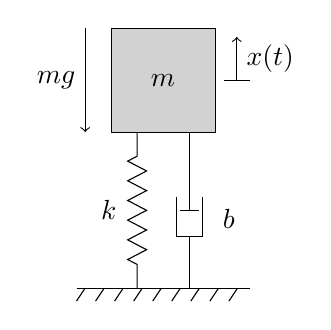
\begin{tikzpicture}[
    scale=1.1,
    spring/.style={decorate, decoration={zigzag, pre length=0.3cm, post length=0.3cm, segment length=0.25cm, amplitude=0.12cm}},
]
  % ---- car body (mass) ----
  \fill[gray!35] (-0.6,1.8) rectangle (0.6,3.0);
  \draw (-0.6,1.8) rectangle (0.6,3.0);
  \node at (0,2.4) {$m$};

  % ---- suspension: spring (left) and damper (right), in parallel ----
  \draw[spring] (-0.3,0) -- (-0.3,1.8);
  \node[left=4pt] at (-0.3,0.9) {$k$};
  % damper: piston plate inside an open cup
  \draw (0.3,0) -- (0.3,0.6);
  \draw (0.15,1.05) -- (0.15,0.6) -- (0.45,0.6) -- (0.45,1.05);
  \draw (0.19,0.9) -- (0.41,0.9);
  \draw (0.3,0.9) -- (0.3,1.8);
  \node[right=4pt] at (0.45,0.8) {$b$};

  % ---- ground ----
  \draw (-1.0,0) -- (1.0,0);
  \foreach \i in {0,...,8} { \draw (-0.9+0.22*\i,0) -- (-1.0+0.22*\i,-0.15); }

  % ---- displacement and force arrows ----
  \draw (0.7,2.4) -- (1.0,2.4);
  \draw[->] (0.85,2.4) -- (0.85,2.9) node[midway,right] {$x(t)$};
  \draw[->] (-0.9,3.0) -- (-0.9,1.8) node[midway,left] {$mg$};
\end{tikzpicture}
\end{center}
